\documentclass[11pt]{article}
\usepackage[utf8]{inputenc}
\usepackage[myheadings]{fullpage}
% \DeclareUnicodeCharacter{0301}{\hspace{-1ex}\'{ }}
% Package for headers 
\usepackage{lastpage}

% For figures and stuff
%\usepackage{graphicx, wrapfig, subcaption, setspace, booktabs}
\usepackage{subcaption}
\usepackage[T1]{fontenc}
\usepackage{lmodern}
\usepackage[protrusion=true, expansion=true]{microtype}

% Change for different font sizes and families
\usepackage[font=small, labelfont=bf]{caption}
% \usepackage{fourier}

% Maths
\usepackage{amsmath,amssymb}
\usepackage{float}
\usepackage{graphicx}
% \usepackage[colorinlistoftodos]{todonotes}
\usepackage[colorlinks=true, allcolors=blue]{hyperref}

% Bibliography
\usepackage{biblatex} 
\addbibresource{references.bib}

%% Language and font encodings
\usepackage[brazil]{babel}
\usepackage{csquotes}

\usepackage{booktabs}
\newcommand{\HRule}[1]{\rule{\linewidth}{#1}}

\setcounter{tocdepth}{5}
\setcounter{secnumdepth}{5}

%% Sets page size and margins
\usepackage[a4paper,top=2cm,bottom=1.5cm,left=2cm,right=2cm,marginparwidth=1.5cm]{geometry}

% Header and footer information
\setlength\headheight{15pt}

 \setlength {\marginparwidth }{2cm}
\begin{document}

\date{}

% Do not change anything here except in \LARGE \textbf{This is the title of the essay} 
% /hline before and after the title makes those horoziontal lines appear, you can change the appearance by changing the 2pt to different sizees
\title{ \normalsize Universidade Federal de São João del-Rei
		\\ [1.0cm]
		% Change to your faculty if needed
		
\includegraphics[width=25mm]{img/ufsjbr_logo.jpg}  \\[.5cm]
		\normalsize Ciência da Computação \\ [3.5cm]
		\HRule{2pt} \\
		\LARGE \textbf{Análise e Classificação de Doenças da Tireoide com XGBoost} %para que quede encerrado en las lineas
		\HRule{2pt} \\ [0.5cm]
		\normalsize \today \vspace*{5\baselineskip}}
		
\date{}

\author{
        Relatório de Mineração de Dados \\[0.5cm]
		Kariny Abrahão (212050013)            \\[1cm]
		 Professor:        \\
		 Leonardo Rocha
		 }
		 
\maketitle

\newpage

\tableofcontents

\section{Introdução}
A glândula tireoide desempenha um papel fundamental na regulação do metabolismo humano por meio da produção dos hormônios triiodotironina (T3) e tiroxina (T4). Alterações no funcionamento dessa glândula podem gerar duas condições clínicas principais: \textbf{hipotireoidismo} e \textbf{hipertireoidismo}.  
O \textbf{hipotireoidismo} ocorre quando há uma produção insuficiente de hormônios tireoidianos, o que pode levar a sintomas como fadiga, ganho de peso, intolerância ao frio e depressão. Já o \textbf{hipertireoidismo} é caracterizado pelo excesso de hormônios tireoidianos, causando perda de peso não intencional, ansiedade, taquicardia e intolerância ao calor. Ambas as condições, quando não diagnosticadas ou tratadas adequadamente, podem comprometer significativamente a qualidade de vida dos pacientes e até gerar complicações mais graves.  
Na prática clínica, o diagnóstico dessas disfunções é realizado principalmente pela análise de exames laboratoriais. O \textbf{TSH (hormônio estimulador da tireoide)} é considerado o marcador mais sensível: níveis elevados de TSH sugerem \textbf{hipotireoidismo}, enquanto níveis suprimidos (muito baixos) indicam \textbf{hipertireoidismo}. Além disso, a dosagem dos hormônios tireoidianos T3 e T4 auxilia na confirmação do quadro: no hipotireoidismo observa-se T4 reduzido, enquanto no hipertireoidismo os níveis de T3 e T4 costumam estar aumentados. Outros índices derivados, como o \textbf{FTI (Free Thyroxine Index)} e o \textbf{T4U (T4 uptake)}, também são utilizados para refinar a interpretação.  
Apesar de bem estabelecidos na prática médica, esses exames nem sempre apresentam cortes claros entre as diferentes condições, havendo sobreposição de valores entre indivíduos saudáveis e doentes. Esse cenário torna o diagnóstico desafiador em alguns casos, principalmente quando existem valores limítrofes ou resultados laboratoriais inconsistentes.  
Nesse contexto, técnicas de \textbf{mineração de dados e aprendizado de máquina} vêm sendo exploradas como ferramentas de apoio ao diagnóstico de doenças da tireoide. Essas técnicas permitem lidar com grandes conjuntos de dados, aplicar estratégias de pré-processamento para tratar inconsistências e treinar modelos de classificação capazes de distinguir entre indivíduos saudáveis, com hipotireoidismo ou com hipertireoidismo.  
O presente trabalho tem como objetivo realizar um estudo de caso utilizando a base de dados \textit{Thyroid Disease Data}, disponível no Kaggle \cite{thyroid-dataset} para responder:

\newpage
% Research Question
%\HRule{0.5pt}\\
\par\noindent\rule{\textwidth}{0.4pt}
\begin{center}
    \textit{Como técnicas de aprendizado de máquina, em especial o XGBoost, podem auxiliar no diagnóstico automatizado de doenças da tireoide (hipotireoidismo e hipertireoidismo) a partir de exames laboratoriais?}
\end{center}
\par\noindent\rule{\textwidth}{0.4pt}
%\HRule{0.5pt}\\

 
\section{Atividades Práticas}

Durante o desenvolvimento deste trabalho prático, foram realizadas as seguintes atividades:

\begin{itemize}
    \item Pesquisa bibliográfica sobre doenças da tireoide (hipotireoidismo e hipertireoidismo) e revisão de artigos que utilizam aprendizado de máquina aplicado ao diagnóstico médico.
    \item Seleção e análise inicial dos dados.
    \item Pré-processamento dos dados, análise exploratória dos dados, tratamento de valores, padronização e balanceamento das classes utilizando oversampling \textit{(SMOTE)}.
    \item Implementação do algoritmo XGBoost.
    \item Avaliação do modelo utilizando métricas como acurácia, precisão, recall e f1-score.
    \item Geração de gráficos e visualizações para análise das importâncias das variáveis no modelo.
\end{itemize}

\begin{figure}[H]
    \centering
    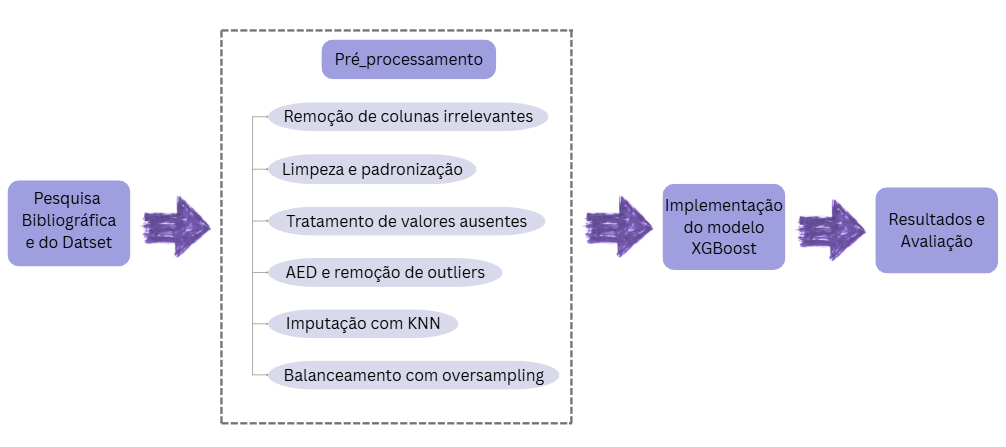
\includegraphics[width=0.8\textwidth]{img/fluxogram.png}
    \caption{Fluxograma resumido das atividades.}
    \label{fig:fluxograma_atividades}
\end{figure}

\subsection{Atividade 1 - Pesquisa bibliográfica}
Para fundamentar o pré-processamento e as técnicas de classificação aplicadas neste trabalho, foram utilizadas como referência diversas fontes, entre notebooks e artigos científicos. Em particular:

\begin{itemize}
  \item Notebooks do Kaggle, como “XGBoost Multi-Class Classification” de EmmanuelFwerr, “Thyroid Disease Detection” de iamArslanKhalid, e “Thyroid Classification” de ZiadAbdelaziz, que fornecem exemplos práticos de análise exploratória de dados (EDA), tratamento de valores ausentes, encoding e avaliação com métricas variadas.
  \item O artigo “\textit{Enhanced Diagnosis of Thyroid Diseases Through Advanced Machine Learning Methodologies}” (Oture, Iqbal \& Wang, 2025), que compara várias técnicas de ML e DL aplicadas ao mesmo tipo de dados, ressaltando uso de oversampling/undersampling e identificando TSH como biomarcador importante.\cite{oture2025enhanced}
  \item “\textit{The novel self-stack ensemble model for thyroid disease prediction}”\cite{Ji2024_SSC_Thyroid}, que desenvolve um modelo de ensemble auto-empilhado (SSC) com técnicas de reamostragem para lidar com desbalanceamento de classes;
  \item O trabalho de Gupta et al. (2024)\cite{Gupta2024}, que propõe o uso de Differential Evolution para otimização de hiperparâmetros e CTGAN para geração de dados sintéticos, contribuindo para lidar com o problema de desbalanceamento das classes.
  \item O artigo “\textit{Machine Learning Techniques for the Classification of Thyroid Disease}” (Moharekar, Vadar \& Pol, 2024), que compara técnicas de classificação como regressão logística e SVM no mesmo dataset utilizado neste trabalho, alcançando desempenho competitivo.\cite{Moharekar2024} 
\end{itemize}
Essas referências ajudaram a definir escolhas no meu pipeline, como quais variáveis manter, quais métricas observar, como tratar valores ausentes e como balancear classes para evitar viés no modelo.

\subsection{Atividade 2 - Seleção e Análise Exploratória Inicial dos Dados}
A segunda atividade teve como objetivo compreender melhor o conjunto de dados \textit{Thyroid Disease Data}, disponível no Kaggle \cite{thyroid-dataset}, que contém informações clínicas e laboratoriais de pacientes, incluindo variáveis contínuas e categóricas. O dataset possui 9172 registros, quantidade considerada suficiente para a condução de nosso estudo, permitindo a exploração de padrões relevantes e o treinamento de modelos de aprendizado de máquina com validade estatística.
O foco dessa etapa foi detalhar cada uma das features, entendendo o significado de seus valores e como elas poderiam impactar os diagnósticos médicos. 
A Tabela \ref{tab:features} apresenta a descrição das colunas do dataset e os tipos de valores que elas contêm.
A coluna \textbf{target} contém os diagnósticos médicos dos pacientes, que estão detalhados na Tabela \ref{tab:target}.  
Neste estágio, com a ajuda da análise detalhada das features, avaliamos o conjunto de dados e concluímos que ele é suficiente e adequado para o objetivo deste trabalho, que consiste no diagnóstico automatizado de hipotireoidismo e hipertireoidismo.


\begin{table}[H]
\centering
\caption{Descrição das variáveis do conjunto de dados \textit{Thyroid Disease Data}.}
\label{tab:features}
\begin{tabular}{|l|p{10cm}|}
\hline
\textbf{Variável} & \textbf{Descrição} \\ \hline
age & Idade do paciente (inteiro) \\ \hline
sex & Sexo com o qual o paciente se identifica (string) \\ \hline
on\_thyroxine & Se o paciente está em uso de tiroxina (booleano) \\ \hline
query\_on\_thyroxine & Se o paciente acredita estar em uso de tiroxina (booleano) \\ \hline
on\_antithyroid\_meds & Se o paciente está em uso de medicamentos antitireoidianos (booleano) \\ \hline
sick & Se o paciente está doente (booleano) \\ \hline
pregnant & Se o paciente está grávida (booleano) \\ \hline
thyroid\_surgery & Se o paciente já passou por cirurgia na tireoide (booleano) \\ \hline
I131\_treatment & Se o paciente está em tratamento com I131 (booleano) \\ \hline
query\_hypothyroid & Se o paciente acredita ter hipotireoidismo (booleano) \\ \hline
query\_hyperthyroid & Se o paciente acredita ter hipertireoidismo (booleano) \\ \hline
lithium & Se o paciente faz uso de lítio (booleano) \\ \hline
goitre & Se o paciente apresenta bócio (booleano) \\ \hline
tumor & Se o paciente possui tumor (booleano) \\ \hline
hypopituitary & Se o paciente apresenta hipopituitarismo (booleano) \\ \hline
psych & Se o paciente apresenta condição psiquiátrica (booleano) \\ \hline
TSH\_measured & Se o TSH foi medido no sangue (booleano) \\ \hline
TSH & Nível de TSH no sangue a partir de exame laboratorial (float) \\ \hline
T3\_measured & Se o T3 foi medido no sangue (booleano) \\ \hline
T3 & Nível de T3 no sangue a partir de exame laboratorial (float) \\ \hline
TT4\_measured & Se o TT4 foi medido no sangue (booleano) \\ \hline
TT4 & Nível de TT4 no sangue a partir de exame laboratorial (float) \\ \hline
T4U\_measured & Se o T4U foi medido no sangue (booleano) \\ \hline
T4U & Nível de T4U no sangue a partir de exame laboratorial (float) \\ \hline
FTI\_measured & Se o FTI foi medido no sangue (booleano) \\ \hline
FTI & Nível de FTI no sangue a partir de exame laboratorial (float) \\ \hline
TBG\_measured & Se o TBG foi medido no sangue (booleano) \\ \hline
TBG & Nível de TBG no sangue a partir de exame laboratorial (float) \\ \hline
referral\_source & Fonte de encaminhamento do paciente (string) \\ \hline
target & Diagnóstico médico (string) \\ \hline
patient\_id & Identificador único do paciente (string) \\ \hline
\end{tabular}
\end{table}

\begin{table}[H]
\centering
\caption{Descrição dos códigos de diagnóstico presentes na coluna \textit{target}.}
\label{tab:target}
\begin{tabular}{ll}
\toprule
\textbf{Letra} & \textbf{Diagnóstico} \\
\midrule
\multicolumn{2}{l}{\textit{Condições de hipertireoidismo}} \\
A & Hipertireoidismo \\
B & T3 tóxico \\
C & Bócio tóxico \\
D & Tóxico secundário \\
\midrule
\multicolumn{2}{l}{\textit{Condições de hipotireoidismo}} \\
E & Hipotireoidismo \\
F & Hipotireoidismo primário \\
G & Hipotireoidismo compensado \\
H & Hipotireoidismo secundário \\
\midrule
\multicolumn{2}{l}{\textit{Proteína de ligação}} \\
I & Proteína de ligação aumentada \\
J & Proteína de ligação diminuída \\
\midrule
\multicolumn{2}{l}{\textit{Saúde geral}} \\
K & Doença não tireoidiana concomitante \\
\midrule
\multicolumn{2}{l}{\textit{Terapia de reposição}} \\
L & Consistente com terapia de reposição \\
M & Sub-reposição \\
N & Super-reposição \\
\midrule
\multicolumn{2}{l}{\textit{Tratamento antitireoidiano}} \\
O & Medicamentos antitireoidianos \\
P & Tratamento com I131 \\
Q & Cirurgia \\
\midrule
\multicolumn{2}{l}{\textit{Diversos}} \\
R & Resultados de exames discordantes \\
S & TBG elevado \\
T & Hormônios tireoidianos elevados \\
\bottomrule
\end{tabular}
\end{table}

\subsection{Atividade 3 - Pré-processamento, Balanceamento dos Dados e Análise Exploratória}
Após a análise inicial, iniciou-se o pré-processamento dos dados, etapa fundamental para garantir que o modelo de aprendizado de máquina pudesse ser treinado de forma eficaz. As ações realizadas incluíram:

\subsubsection{Remoção de colunas redundantes e irrelevantes}
O primeiro passo no pré-processamento foi analisar a relevância de cada coluna do dataset. Colunas do tipo \texttt*\_measured foram removidas, pois indicavam apenas se um exame havia sido realizado e não forneciam informação adicional relevante para o modelo. A coluna \texttt{patient\_id}, por se tratar de um identificador único, também foi descartada por não possuir utilidade preditiva. Da mesma forma, a coluna \texttt{referral\_source} foi removida, por não agregar valor significativo na previsão do diagnóstico. Por fim, a coluna \texttt{TBG} foi excluída, uma vez que apresentava uma quantidade extremamente elevada de valores nulos (8823 de 9172, aproximadamente 96\%) e não é considerada fundamental para os diagnósticos de hipotireoidismo ou hipertireoidismo.
Essas remoções simplificaram o dataset, reduziram a complexidade do modelo e eliminaram colunas que poderiam introduzir ruído ou viés desnecessário.

\subsubsection{Limpeza e padronização da variável target}
Posteriormente, iniciamos a exploração e limpeza da variável \textbf{target}, que representa o alvo do modelo. Primeiramente, foram removidos espaços em branco e todas as letras foram padronizadas para maiúsculas, evitando erros ou perda de informação.  
Em seguida, filtramos apenas os diagnósticos relevantes para o estudo: as letras que representam o hipertireoidismo (A, B, C, D), o hipotireoidismo (E, F, G, H), e os casos negativos, representados pelo caractere "\texttt{-}". Todas as demais linhas contendo outros diagnósticos foram removidas, a fim de evitar ruídos e possíveis vieses no modelo.  
Por fim, a coluna \textbf{target} foi mapeada numericamente: 0 para os casos negativos, 1 para o hipotireoidismo e 2 para o hipertireoidismo, tornando-a adequada para o treinamento do modelo de classificação.

\subsubsection{Tratamento de valores ausentes}
Inicialmente, foram preenchidos alguns valores ausentes na coluna \texttt{sex}. Para os casos em que o sexo estava nulo, verificou-se a coluna \texttt{pregnant}: quando o valor era verdadeiro, atribuiu-se diretamente o sexo feminino, já que a condição de gravidez não seria possível para indivíduos do sexo masculino.
Além disso, utilizando o parâmetro \texttt{thresh=18} na função \texttt{dropna}, de forma a remover linhas que continham mais de quatro valores ausentes (dado que havia um total de 22 atributos, incluindo a variável alvo). Esse procedimento eliminou instâncias incompletas que poderiam comprometer a qualidade do modelo, ao mesmo tempo este procedimento resultou indiretamente em uma redução da classe majoritária (0), funcionando de forma semelhante a uma técnica de \textit{undersampling} não intencional, o que contribuiu para melhorar o balanceamento do conjunto de dados.
Na Figura~\ref{fig:pie-before-after}, observa-se a distribuição das classes antes e após a aplicação do filtro de valores nulos. Nota-se a queda da classe negativa (0) e a elevação proporcional das classes de hipotireoidismo (1) e hipertireoidismo (2), contribuindo para um balanceamento mais adequado do conjunto de dados.

\begin{figure}[H]
    \centering
    \subfloat[Distribuição antes do filtro (thresh=18)]{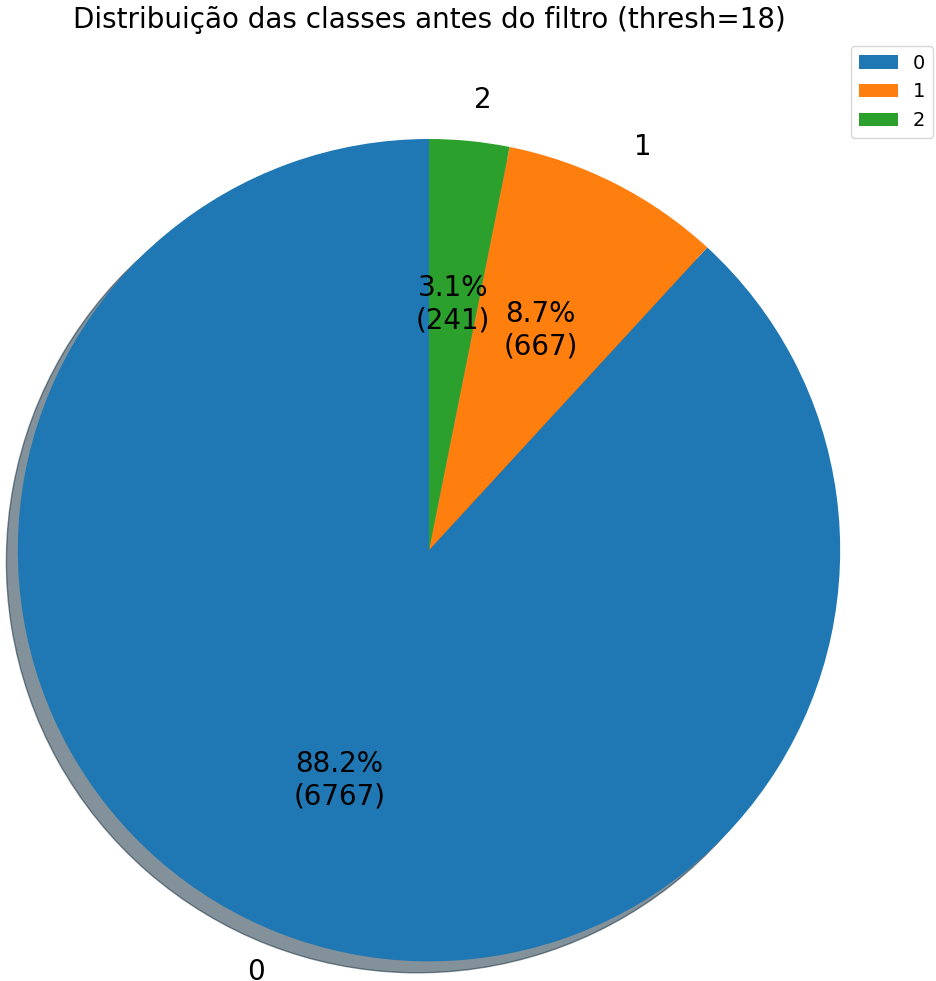
\includegraphics[width=0.50\textwidth]{img/pie_before.png}}
    \hfill
    \subfloat[Distribuição após o filtro (thresh=18)]{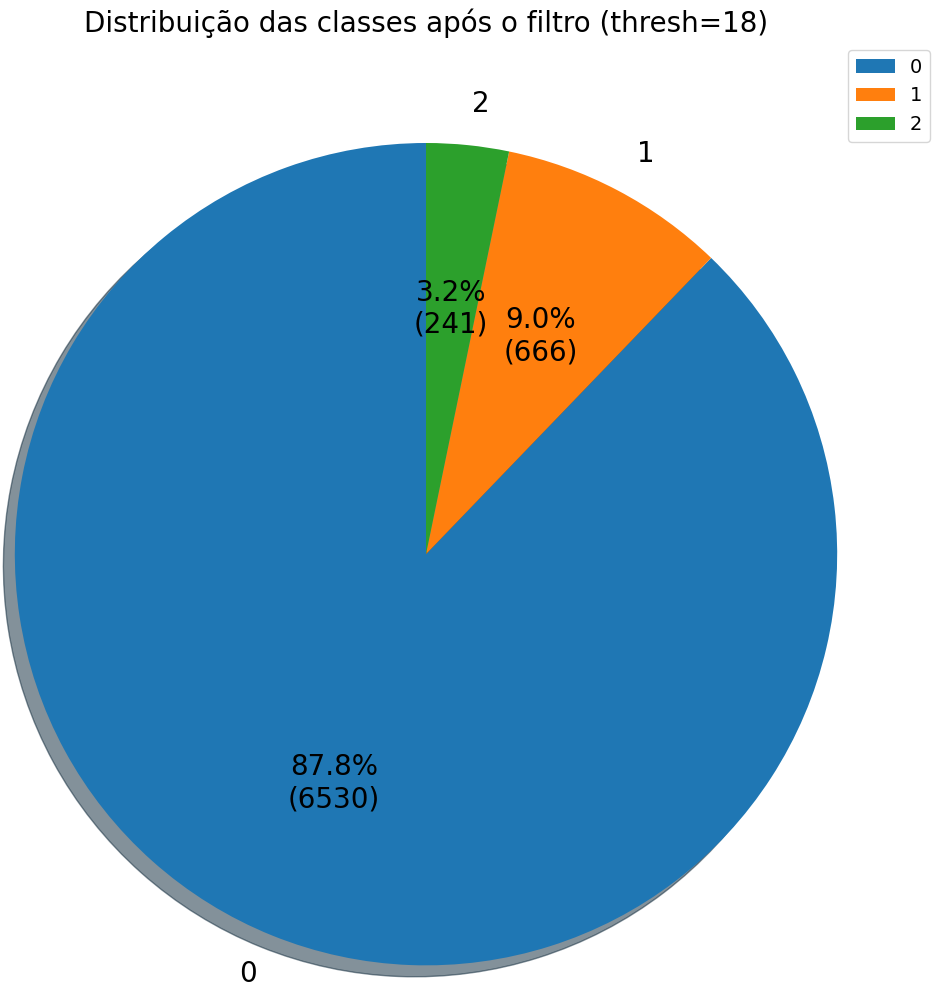
\includegraphics[width=0.50\textwidth]{img/pie_after.png}}
    \caption{Distribuição das classes antes e depois da aplicação do filtro de valores nulos.}
    \label{fig:pie-before-after}
\end{figure}

\subsubsection{Análise exploratória e remoção de outliers}

Para entender melhor a distribuição das variáveis numéricas em relação ao \textit{target}, foram gerados gráficos de dispersão (\textit{strip plots}) para cada atributo numérico, com cores diferenciando as classes do \textit{target} (0 = outros, 1 = hipotireoidismo, 2 = hipertireoidismo). 
Os gráficos permitiram identificar valores extremos em algumas colunas, o que possibilitou a definição de limites plausíveis para cada variável. Dessa forma, foram impostas restrições nos dados numéricos para remover outliers e evitar que valores atípicos viessem a enviesar o modelo. Os limites aplicados foram:

\begin{itemize}
    \item \textbf{TSH}: 0 -- 500
    \item \textbf{T3}: 0 -- 20
    \item \textbf{TT4}: 0 -- 400
    \item \textbf{T4U}: 0 -- 2
    \item \textbf{FTI}: 0 -- 300
    \item \textbf{Idade}: 0 -- 100 anos
\end{itemize}

A Figura \ref{fig:stripplots} apresenta os gráficos gerados, onde cada ponto representa um paciente e as cores indicam a classe do \textit{target}. Observa-se que a aplicação desses limites contribuiu para remover valores extremos que poderiam impactar negativamente o desempenho do modelo de classificação.

\begin{figure}[H]
    \centering
    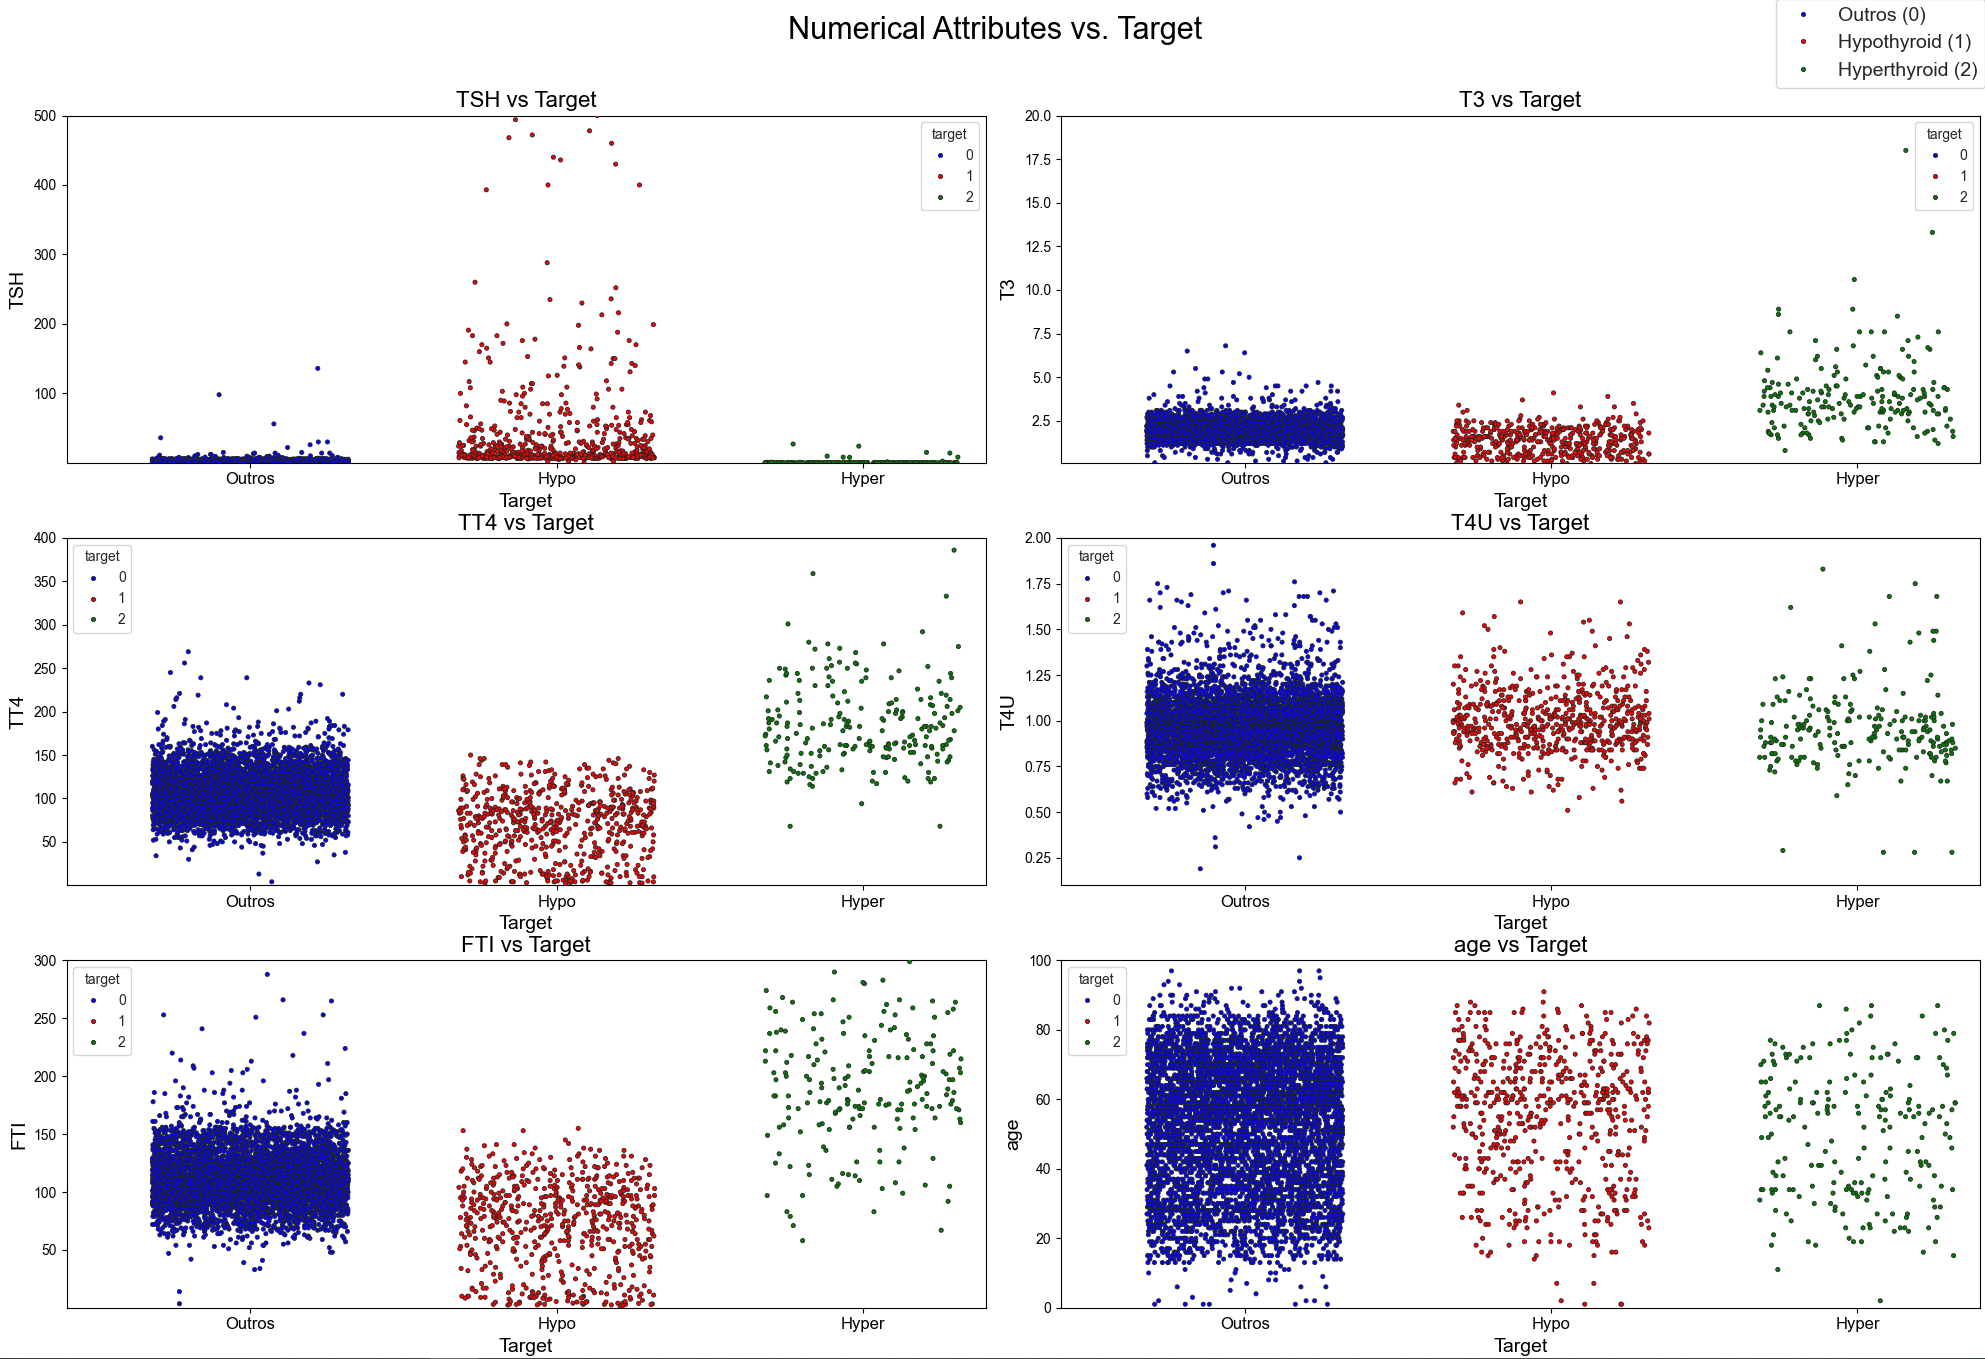
\includegraphics[width=1.0\textwidth]{img/numerical_stripplots.png}
    \caption{Distribuição das variáveis numéricas em função do \textit{target}, com limites aplicados para remoção de outliers.}
    \label{fig:stripplots}
\end{figure}

\subsubsection{Imputação de valores nulos utilizando KNN}

Após a remoção de outliers e a análise das variáveis, foi realizada a imputação dos valores nulos restantes utilizando o método de KNN (\textit{K-Nearest Neighbors}). Para isso, considerou-se os 10 vizinhos mais próximos de cada registro, atribuindo pesos maiores aos vizinhos mais próximos. Esse procedimento permitiu preencher tanto os valores nulos das variáveis numéricas quanto das categóricas, preservando a estrutura dos dados.
Antes da aplicação do KNN, foi necessário transformar as variáveis categóricas, que possuíam valores binários como ``t''/``f'' ou ``0''/``1'', para um formato adequado, garantindo que o algoritmo pudesse processá-las corretamente.
Para analisar o impacto da imputação, foram geradas curvas de distribuição das principais variáveis contínuas (\textbf{TSH}, \textbf{T3}, \textbf{TT4}, \textbf{T4U}, \textbf{FTI}) antes e depois do KNN. As figuras \ref{fig:FTI_distrib} a \ref{fig:T4U_distrib} apresentam essas distribuições. Observa-se que, embora a curva do dado original tenha ficado ligeiramente abaixo da curva após a imputação, o formato geral das distribuições se manteve, indicando que a imputação preservou a característica dos dados sem introduzir distorções significativas.

\begin{figure}[H]
    \centering
    \begin{minipage}{0.48\textwidth}
        \centering
        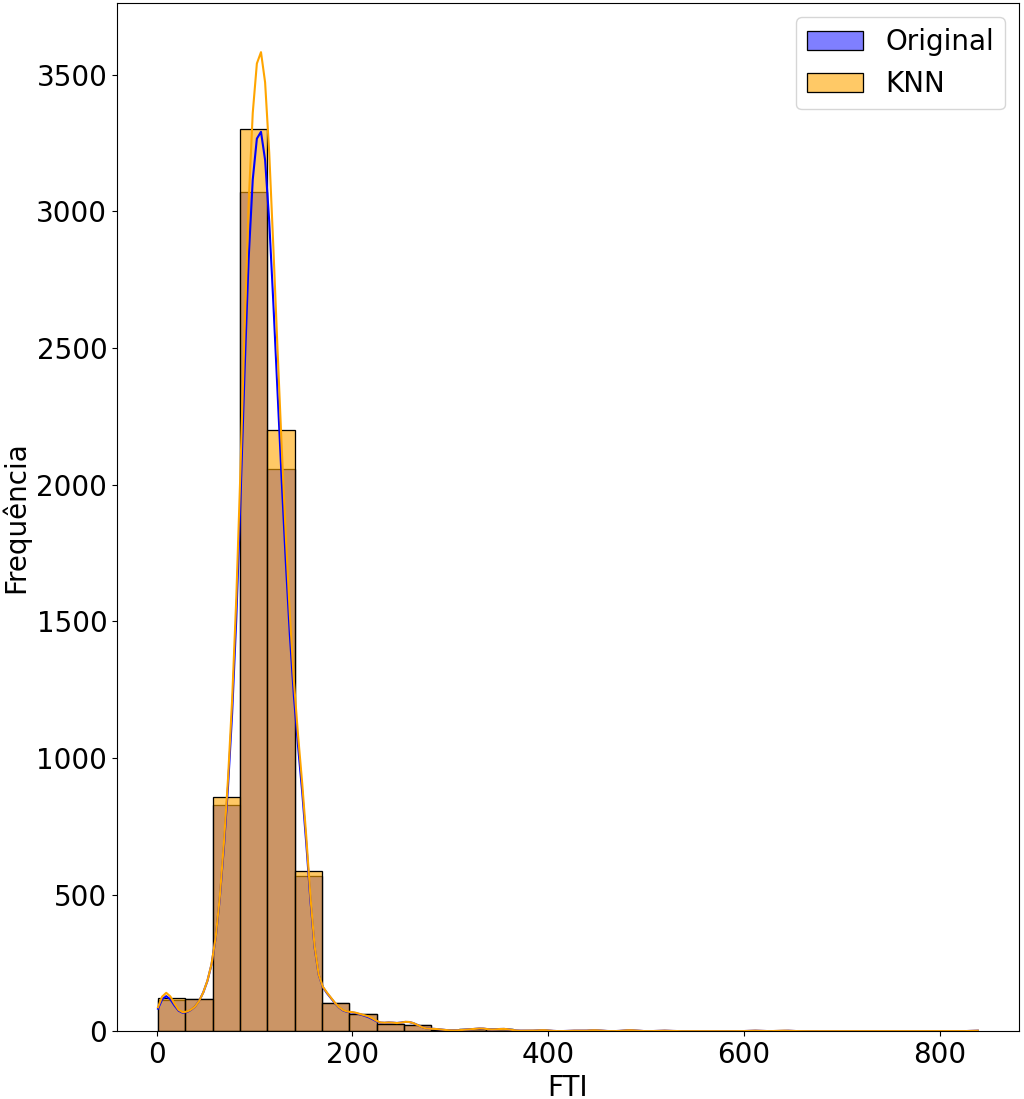
\includegraphics[width=\textwidth]{img/FTI_distrib.png}
        \caption{Distribuição da variável FTI.}
        \label{fig:FTI_distrib}
    \end{minipage}
    \hfill
    \begin{minipage}{0.48\textwidth}
        \centering
        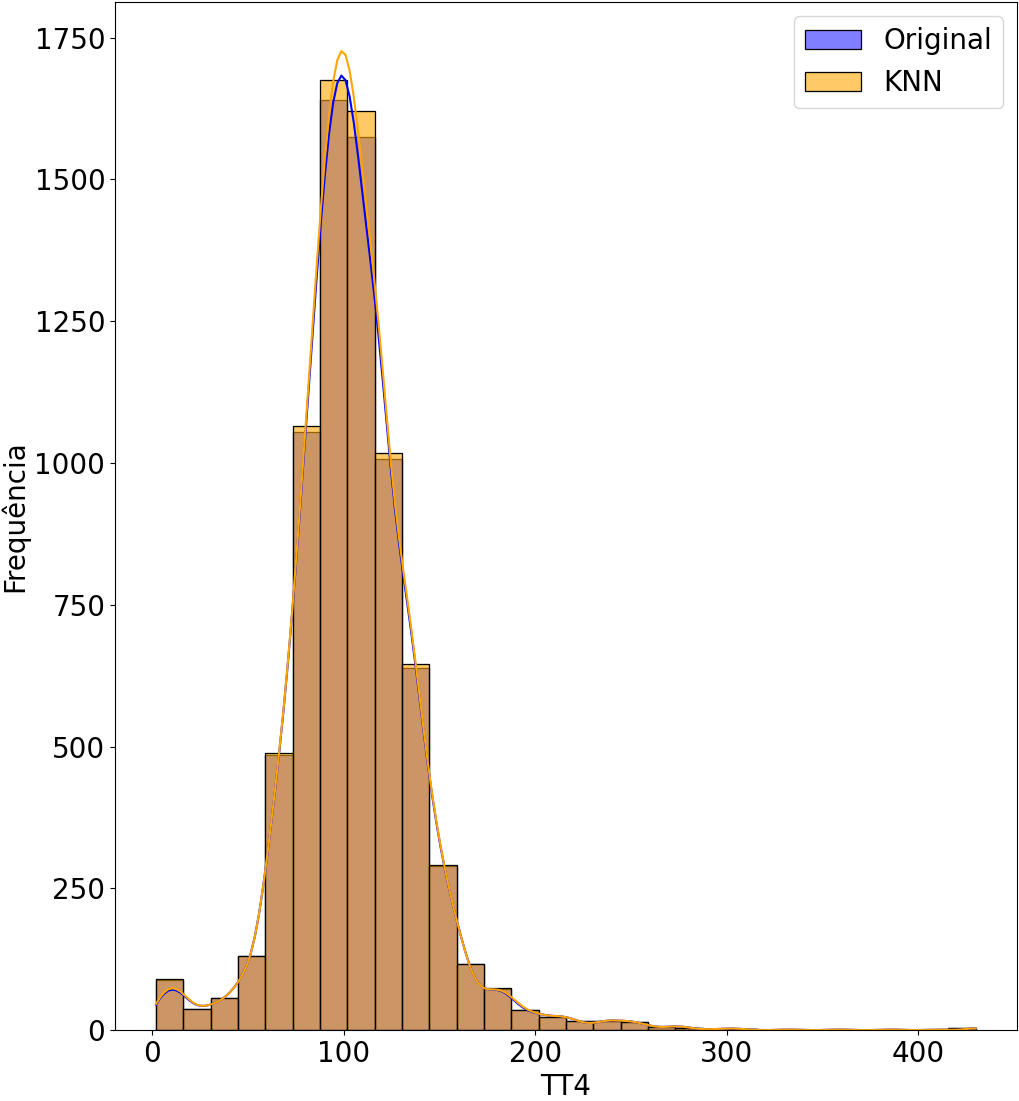
\includegraphics[width=\textwidth]{img/TT4_distrib.png}
        \caption{Distribuição da variável TT4.}
        \label{fig:TT4_distrib}
    \end{minipage}
\end{figure}

\begin{figure}[H]
    \centering
    \begin{minipage}{0.48\textwidth}
        \centering
        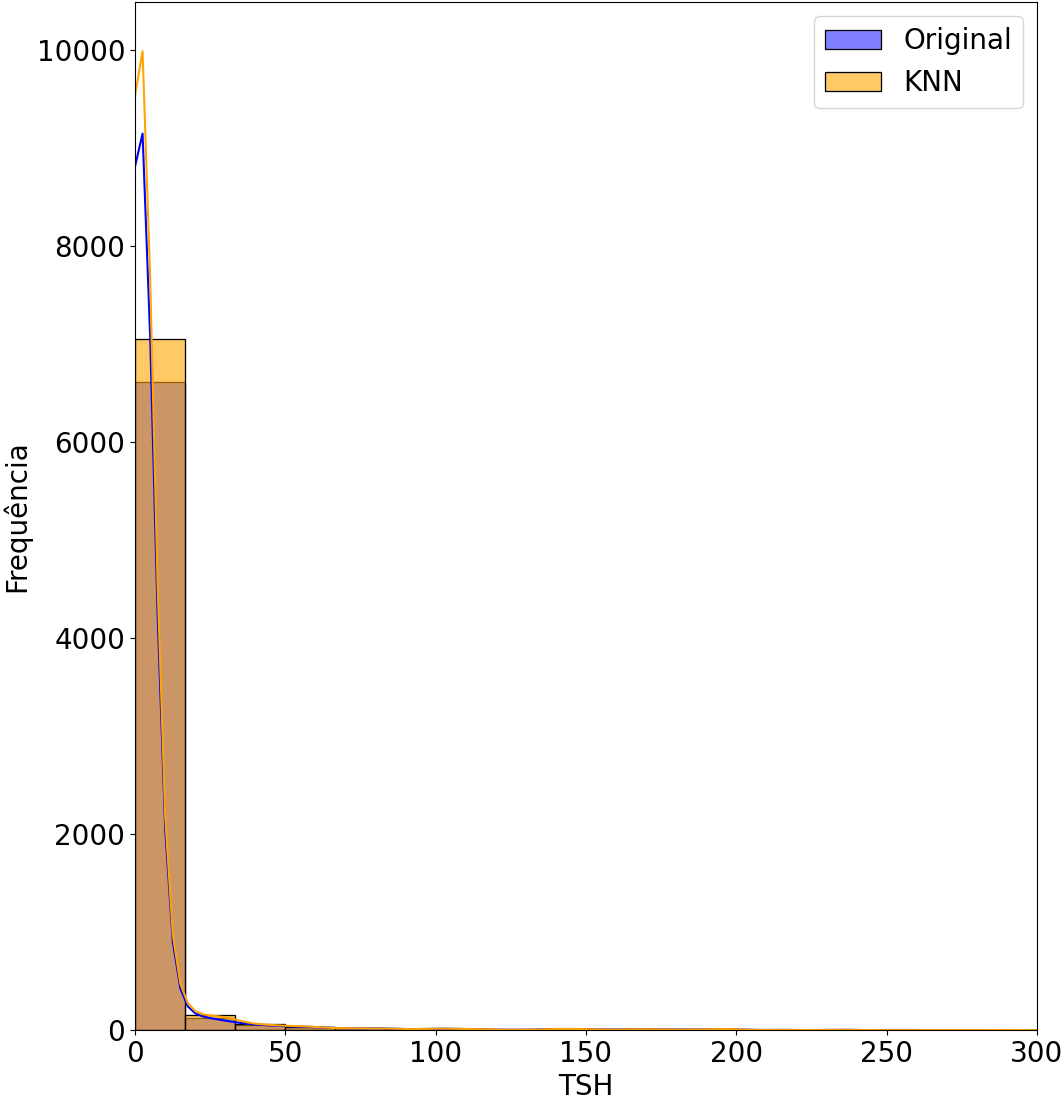
\includegraphics[width=\textwidth]{img/TSH_distrib.png}
        \caption{Distribuição da variável TSH.}
        \label{fig:TSH_distrib}
    \end{minipage}
    \hfill
    \begin{minipage}{0.48\textwidth}
        \centering
        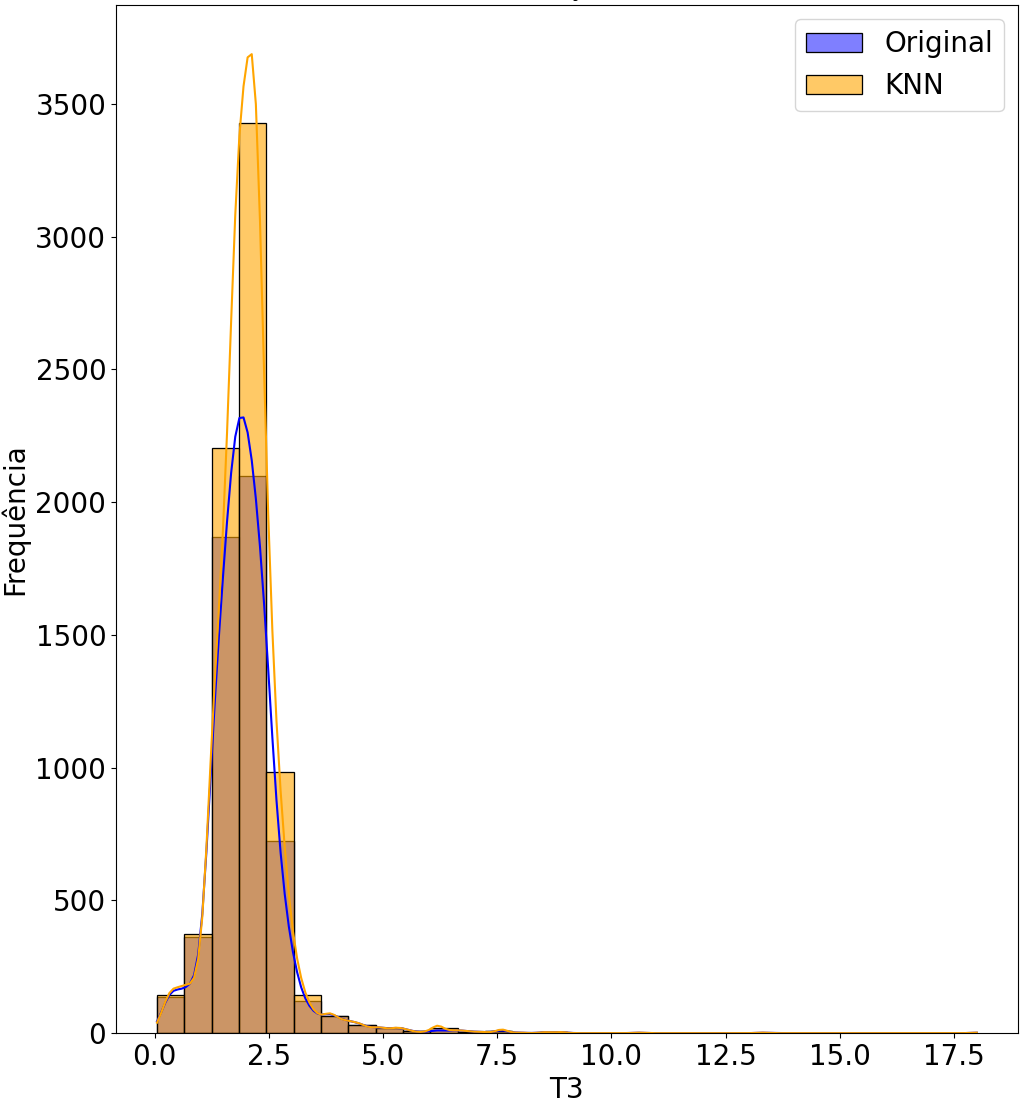
\includegraphics[width=\textwidth]{img/T3_distrib.png}
        \caption{Distribuição da variável T3.}
        \label{fig:T3_distrib}
    \end{minipage}
\end{figure}

\begin{figure}[H]
    \centering
    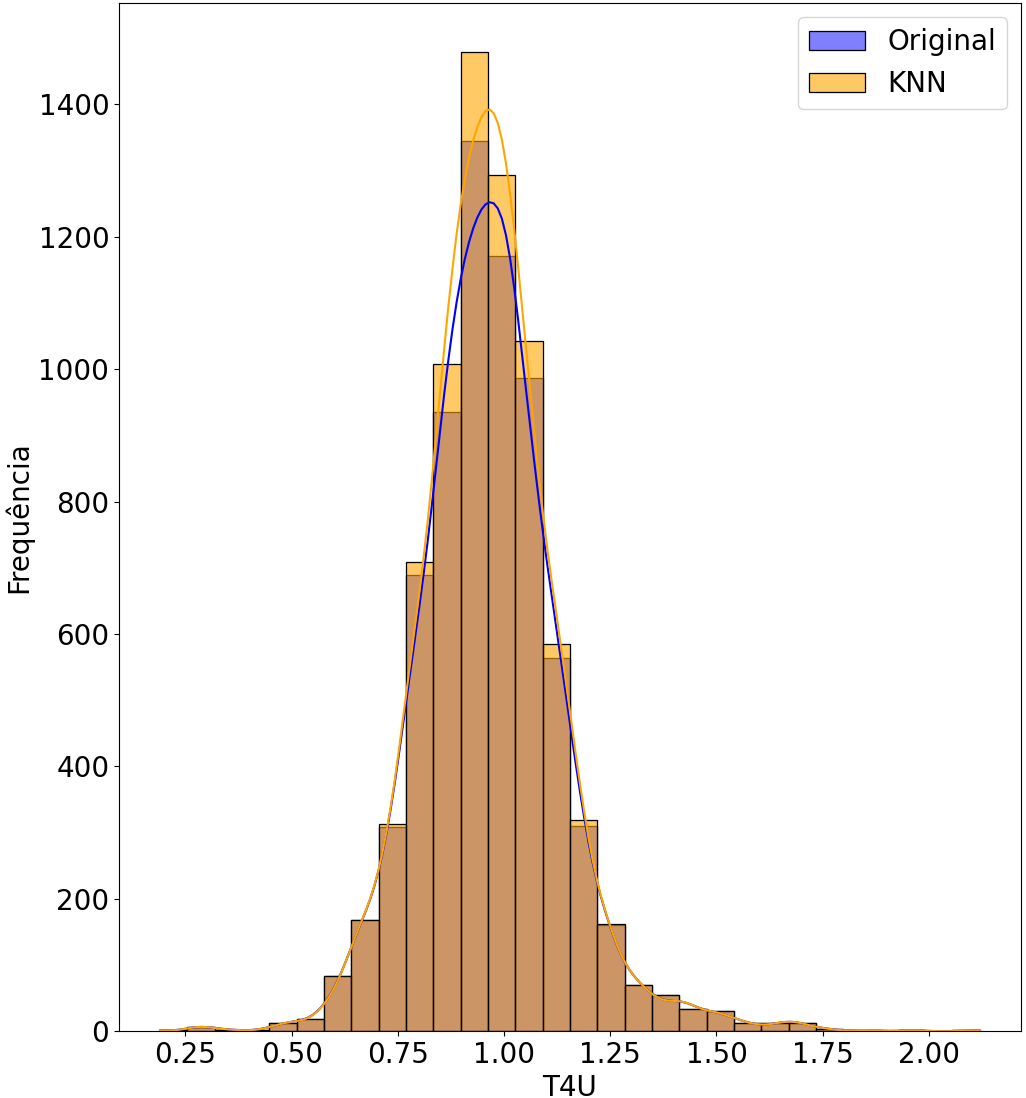
\includegraphics[width=0.4\textwidth]{img/T4U_distrib.png}
    \caption{Distribuição da variável T4U.}
    \label{fig:T4U_distrib}
\end{figure}

\subsubsection{Balanceamento das classes com SMOTE}

Após a divisão inicial dos dados em treino e teste, com 33\% reservados para avaliação, foi aplicado o método \textit{SMOTE (Synthetic Minority Over-sampling Technique)} ao conjunto de treino. A função \texttt{train\_test\_split} do \texttt{scikit-learn} foi utilizada com o parâmetro \texttt{stratify=y} para garantir que a proporção de cada classe fosse mantida em ambos os conjuntos.

O \textit{SMOTE} é uma técnica de oversampling que cria amostras sintéticas das classes minoritárias, de modo a balancear o conjunto de treino e permitir que o modelo aprenda melhor padrões de todas as classes. O parâmetro \texttt{random\_state=44} foi definido para tornar o processo reprodutível.  

\subsubsection{Implementação do XGBoost}

Para a etapa final do estudo de caso, foi implementado um modelo \textit{XGBoost} para classificação dos pacientes em três classes: negativos, hipotireoidismo e hipertireoidismo. Inicialmente, buscou-se otimizar os hiperparâmetros do modelo utilizando \textit{GridSearchCV}, mas os melhores valores foram definidos manualmente como:

\begin{itemize}
    \item \texttt{colsample\_bytree = 0.7} 
    \item \texttt{learning\_rate = 0.1} 
    \item \texttt{max\_depth = 7} 
    \item \texttt{n\_estimators = 100} 
    \item \texttt{subsample = 1.0} 
    \item \texttt{objective = 'multi:softmax'} 
    \item \texttt{num\_class = 3} 
    \item \texttt{eval\_metric = ['merror', 'mlogloss']}
\end{itemize}

Para lidar com o desbalanceamento das classes, foi utilizado o vetor de \textit{sample\_weight}, calculado a partir da função \texttt{compute\_sample\_weight} com o parâmetro \texttt{class\_weight='balanced'}. Esse vetor ajusta o peso de cada amostra, dando maior importância para as classes minoritárias durante o treinamento.

O modelo foi treinado utilizando o conjunto de treino reamostrado pelo SMOTE e avaliado no conjunto de teste original, preservando a distribuição real das classes.  

\section{Resultados}

Após a implementação do modelo XGBoost, foi realizada a avaliação de desempenho e análise da importância das features. O modelo foi treinado utilizando as amostras balanceadas pelo SMOTE e aplicando o \texttt{sample\_weight} para dar maior peso às classes minoritárias.

\subsection{Importância das Features}

A importância das variáveis foi calculada pelo próprio modelo XGBoost, gerando um ranking que indica quais features mais contribuíram para a predição. Observou-se que, antes da utilização do \texttt{sample\_weight}, a feature de maior importância era o \textbf{FTI}. Após aplicar os pesos para equilibrar as classes, a feature mais importante passou a ser o \textbf{TSH}, alinhando-se melhor com achados reportados na literatura.

\begin{figure}[H]
    \centering
    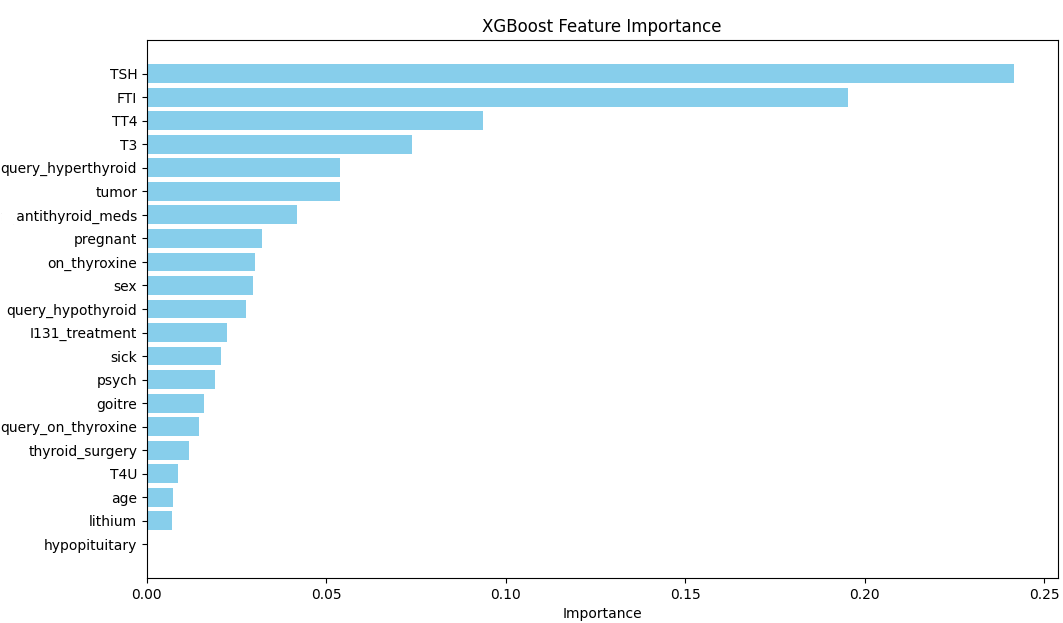
\includegraphics[width=0.7\textwidth]{img/feature_importance.png}
    \caption{Importância das features calculada pelo XGBoost.}
    \label{fig:feature_importance}
\end{figure}

\subsection{Evolução do Treinamento}

O desempenho durante o treinamento foi monitorado pelas métricas de logloss e erro de classificação (\texttt{merror}) para o conjunto de treino e teste.

\begin{figure}[H]
    \centering
    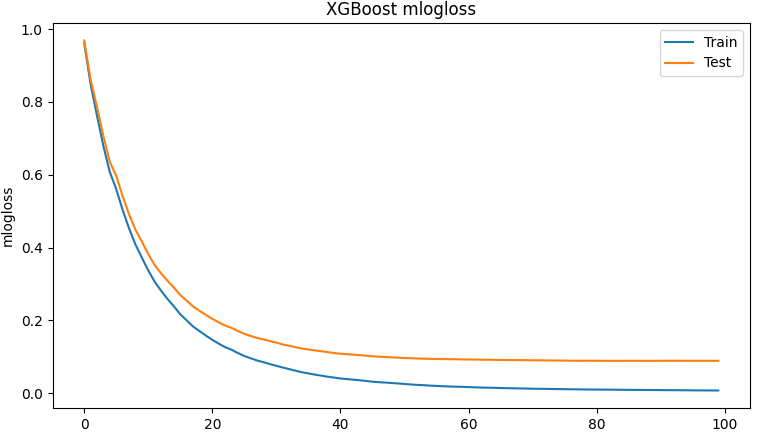
\includegraphics[width=0.7\textwidth]{img/mlogloss.png}
    \caption{Evolução do \texttt{mlogloss} durante o treinamento do XGBoost.}
    \label{fig:mlogloss}
\end{figure}

\begin{figure}[H]
    \centering
    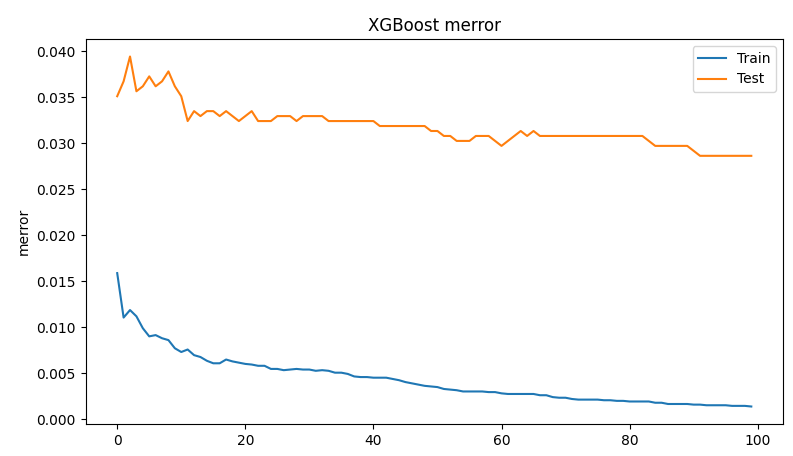
\includegraphics[width=0.7\textwidth]{img/merror.png}
    \caption{Evolução do \texttt{merror} durante o treinamento do XGBoost.}
    \label{fig:merror}
\end{figure}

\subsubsection{Métricas de Avaliação Final}

O modelo foi testado no conjunto de teste, apresentando os seguintes resultados:

\begin{itemize}
    \item \textbf{Accuracy:} 0.97
    \item \textbf{Balanced Accuracy:} 0.96
    \item \textbf{Micro F1-score:} 0.97
    \item \textbf{Macro F1-score:} 0.92
    \item \textbf{Weighted F1-score:} 0.97
\end{itemize}

A matriz de confusão e o relatório de classificação mostraram que o modelo conseguiu identificar de forma consistente os casos de hipotireoidismo e hipertireoidismo, mesmo diante do desbalanceamento inicial das classes.

\begin{figure}[H]
    \centering
    \begin{minipage}{0.48\textwidth}
        \centering
        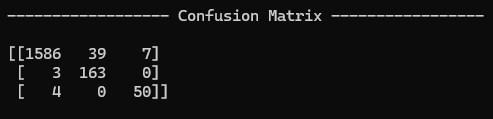
\includegraphics[width=\textwidth]{img/confusion_matrix.png}
        \caption{Matriz de confusão do modelo XGBoost no conjunto de teste.}
        \label{fig:confusion_matrix}
    \end{minipage}%
    \hfill
    \begin{minipage}{0.48\textwidth}
        \centering
        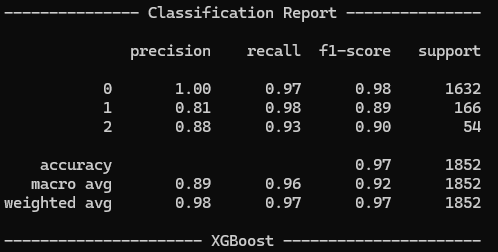
\includegraphics[width=\textwidth]{img/classification_report.png}
        \caption{Relatório de classificação do modelo XGBoost no conjunto de teste.}
        \label{fig:classification_report}
    \end{minipage}
\end{figure}

Em resumo, o modelo XGBoost com ajuste de pesos para as classes minoritárias apresentou resultados satisfatórios para a classificação automatizada das doenças da tireoide, com a importância das features condizente com achados clínicos.

\section{Desafios Encontrados}

Durante o desenvolvimento deste trabalho, alguns desafios se destacaram ao longo das etapas. 
O primeiro desafio esteve relacionado à definição do escopo do projeto e à escolha de um conjunto de dados adequado. Foi necessário um tempo considerável para analisar diferentes bases disponíveis até encontrar o \textit{Thyroid Disease Data}, disponível no Kaggle, que atendia aos requisitos do tema escolhido e possuía informações clínicas e laboratoriais relevantes para o diagnóstico de doenças da tireoide.  
Outro desafio importante foi o estudo das técnicas de pré-processamento e a compreensão da ordem correta em que cada uma deveria ser aplicada. Etapas como a remoção de colunas redundantes, tratamento de valores ausentes com \textit{KNN-Imputer}, filtragem de outliers e balanceamento de classes com \textit{SMOTE} exigiram análise detalhada e testes práticos para garantir que o conjunto de dados final fosse consistente e representativo.  
Além disso, compreender os modelos de classificação e, em particular, o funcionamento do algoritmo XGBoost também representou uma dificuldade inicial. Foi necessário estudar suas bibliotecas, funções e hiperparâmetros de entrada, bem como explorar técnicas complementares como o uso de \textit{GridSearch} para otimização e o cálculo de \textit{sample\_weight} para penalizar erros em classes minoritárias.  
Apesar dessas dificuldades, cada obstáculo contribuiu para um aprendizado significativo, tanto em relação ao uso das ferramentas de aprendizado de máquina quanto na aplicação prática de conceitos de ciência de dados em um contexto real de diagnóstico médico.


\section{Conclusão}

O presente estudo teve como objetivo investigar como técnicas de aprendizado de máquina, em especial o XGBoost, podem auxiliar no diagnóstico automatizado de doenças da tireoide, considerando hipotireoidismo e hipertireoidismo, a partir de exames laboratoriais.
Durante o desenvolvimento do trabalho, foi possível observar que o conjunto de dados \textit{Thyroid Disease Data} do Kaggle, contendo informações clínicas e laboratoriais de 9.172 pacientes, era suficiente e adequado para treinar um modelo de classificação confiável. Por meio de uma etapa sistemática de pré-processamento, que incluiu limpeza de dados, tratamento de valores nulos, padronização e balanceamento das classes com SMOTE, garantiu-se que o modelo fosse treinado com dados de qualidade e representativos.
A implementação do XGBoost, aliada à busca de hiperparâmetros com GridSearch e ao uso de pesos de amostra (\textit{sample\_weight}) para lidar com o desbalanceamento das classes, permitiu identificar corretamente padrões relevantes nos exames laboratoriais. Observou-se que, após aplicar o \textit{sample\_weight}, a importância das variáveis no modelo passou a refletir melhor os achados clínicos descritos na literatura: o TSH tornou-se a variável mais relevante, alinhando-se ao que é considerado um biomarcador sensível para disfunções tireoidianas.
Os resultados obtidos, avaliados por métricas como acurácia, recall, f1-score e análise da matriz de confusão, demonstram que o XGBoost foi capaz de distinguir de forma eficiente entre pacientes saudáveis, hipotireoideos e hipertireoideos. Além disso, a visualização das importâncias das features fornece uma interpretação útil para profissionais de saúde, mostrando quais exames contribuem mais para o diagnóstico automatizado.
Portanto, conclui-se que técnicas de aprendizado de máquina, especialmente o XGBoost, são ferramentas promissoras para o apoio ao diagnóstico de doenças da tireoide. Elas permitem transformar dados laboratoriais em previsões confiáveis, auxiliando médicos a identificar disfunções tireoidianas de forma mais rápida e objetiva, e potencialmente melhorando o cuidado clínico.

\newpage
\printbibliography
\end{document}